\documentclass{article}
\usepackage[T1]{fontenc}
\usepackage[spanish,es-noshorthands]{babel}
\usepackage{adjustbox}
\usepackage{booktabs}
\usepackage{amssymb}
\usepackage{amsmath}
\usepackage{graphicx}
\usepackage{float}
\usepackage{xcolor}
\usepackage[hidelinks]{hyperref}
\usepackage{caption}
\captionsetup{font=small,labelfont=bf}

% generado por hacer_graficas.py: no editar a mano
\newcommand{\NrepsDuno}{457}
\newcommand{\NrepsDdos}{457}
\newcommand{\NrepsDtres}{457}
\newcommand{\NrepsGill}{459}
\newcommand{\ConvDuno}{99.8}
\newcommand{\ConvDdos}{99.8}
\newcommand{\ConvDtres}{100.0}
\newcommand{\ConvGill}{97.6}
\newcommand{\PeorSesgoD}{0.78}
\newcommand{\CobMin}{93.2}
\newcommand{\CobMax}{96.9}
\newcommand{\NrepsEdad}{60}
\newcommand{\NrepsEdadGill}{60}
\newcommand{\ErrPrecioD}{0.50}
\newcommand{\ErrPrecioGillJoven}{1.9}
\newcommand{\PiBarata}{0.50}
\newcommand{\PiBase}{0.42}
\newcommand{\PiCara}{0.32}
\newcommand{\PendLBBarata}{$-$0.013}
\newcommand{\PendLBBase}{$-$0.015}
\newcommand{\PendLBCara}{$-$0.016}
\newcommand{\PendHBBarata}{$-$0.012}
\newcommand{\PendHBBase}{$-$0.007}
\newcommand{\PendHBCara}{$-$0.002}
\newcommand{\Gillmutcero}{$-$40}
\newcommand{\Gillmutuno}{$-$39}
\newcommand{\Gilltcsell}{$-$120}
\newcommand{\Gillucerotcerojcero}{$-$23}
\newcommand{\Gillaccagejcero}{$-$26}
\newcommand{\Gilltcbuytcero}{12}

\addto\captionsspanish{\renewcommand{\tablename}{Tabla}}
% la numeración sigue la lista de gráficas pedida (tablas 1-2, figuras 3-8)

\usepackage{xurl}
\newcommand{\archivo}[1]{\path{#1}}
\sloppy
\newcommand{\nota}[1]{\par\smallskip\noindent\colorbox{black!6}{\parbox{\dimexpr\linewidth-2\fboxsep}{\small\textbf{Ojo.} #1}}\par\smallskip}

\title{Tablas y gráficas de resultados del Monte Carlo\\[2pt]
\large Qué muestran, de qué archivos salen y cómo se calculan}
\author{Generado con \archivo{claude/graphs/hacer_graficas.py}}
\date{22 de noviembre de 2026}

\begin{document}
\maketitle

\tableofcontents

%======================================================================
\section{Cómo está organizada la carpeta y cómo regenerar todo}

Todo está en \archivo{claude/graphs/}:
\begin{itemize}
\item \archivo{hacer_graficas.py}: el único script. Lee los resultados del Monte Carlo, calcula las
  estadísticas, dibuja las figuras, escribe las tablas y compila este documento.
\item \archivo{figuras/}: las figuras en PDF vectorial (\archivo{fig3_dispersion.pdf}, \archivo{fig4_precios.pdf},
  \archivo{fig5_poblacion.pdf}, \archivo{fig6_reparar_edad.pdf}, \archivo{fig7a_mezcla_observada.pdf},
  \archivo{fig7b_componentes.pdf}, \archivo{fig8_reparar_desgaste.pdf}). Están dibujadas con 6 pulgadas de
  ancho y letra de 10\,pt con \LaTeX{} (Computer Modern), para que al meterlas en la tesis a todo
  el ancho del texto la letra combine con la de la tesis.
\item \archivo{tablas/}: \archivo{tab_comunes.tex} y \archivo{tab_propios.tex} (tablas listas para
  \verb|\input|; usan \texttt{booktabs} y \texttt{adjustbox}, que la tesis ya carga),
  \archivo{resumen_parametros.csv} (todas las estadísticas de todos los parámetros y estimadores,
  incluidas las que no salen en las tablas, como el RMSE, el error estándar mediano y la cobertura)
  y \archivo{cifras.tex} (macros con los números que cita este texto, para que se actualicen solos).
\item \archivo{graficas.tex} / \archivo{graficas.pdf}: este documento.
\end{itemize}

Para regenerar todo (por ejemplo, cuando terminen las 1{,}000 réplicas y se haya hecho \texttt{git pull}):
\begin{verbatim}
python -u claude/graphs/hacer_graficas.py           # todo
python -u claude/graphs/hacer_graficas.py --sin_pdf # sin PDF
\end{verbatim}
Tarda alrededor de un minuto. No resuelve ningún equilibrio: las figuras 7 y 8 solo
\emph{evalúan} el modelo en el equilibrio verdadero que ya está guardado (unos segundos en CPU).

\subsection{Para pasarlas a la tesis}
Copiar \archivo{figuras/} y \archivo{tablas/} junto a \archivo{docs/tex/tesis.tex} (o poner la ruta
relativa) y usar, por ejemplo,
\begin{verbatim}
\begin{table}[htbp]
\centering
\small
\setlength{\tabcolsep}{4.5pt}
\begin{adjustbox}{max width=\textwidth}
\begin{tabular}{l r rr rr rr rr}
\toprule
 & & \multicolumn{2}{c}{Gillingham} & \multicolumn{2}{c}{Diseño 1} & \multicolumn{2}{c}{Diseño 2} & \multicolumn{2}{c}{Diseño 3}\\
\cmidrule(lr){3-4} \cmidrule(lr){5-6} \cmidrule(lr){7-8} \cmidrule(lr){9-10}
Parámetro & Verdad & Media & Sesgo \% & Media & Sesgo \% & Media & Sesgo \% & Media & Sesgo \%\\
\midrule
\multicolumn{10}{l}{\textit{Preferencias}}\\
$\mu_{1}$ & 0.113 & 0.068 & \textbf{$-$39.9} & 0.113 & 0.2 & 0.113 & 0.3 & 0.114 & 0.4\\
$\mu_{2}$ & 0.094 & 0.058 & \textbf{$-$38.9} & 0.094 & 0.3 & 0.094 & 0.3 & 0.094 & 0.4\\
$u_{0,1\text{LB}}$ & 3.649 & 2.819 & \textbf{$-$22.7} & 3.654 & 0.1 & 3.655 & 0.2 & 3.657 & 0.2\\
$u_{0,1\text{HB}}$ & 5.154 & 3.626 & \textbf{$-$29.6} & 5.164 & 0.2 & 5.166 & 0.2 & 5.168 & 0.3\\
$u_{0,2\text{LB}}$ & 2.404 & 1.737 & \textbf{$-$27.7} & 2.410 & 0.2 & 2.411 & 0.3 & 2.413 & 0.4\\
$u_{0,2\text{HB}}$ & 3.582 & 2.338 & \textbf{$-$34.7} & 3.593 & 0.3 & 3.595 & 0.4 & 3.597 & 0.4\\
$u_{1,1\text{LB}}$ & $-$0.146 & $-$0.103 & \textbf{29.2} & $-$0.146 & $-$0.1 & $-$0.146 & $-$0.2 & $-$0.146 & $-$0.3\\
$u_{1,1\text{HB}}$ & $-$0.220 & $-$0.166 & \textbf{24.3} & $-$0.220 & $-$0.2 & $-$0.220 & $-$0.2 & $-$0.220 & $-$0.2\\
$u_{1,2\text{LB}}$ & $-$0.098 & $-$0.060 & \textbf{39.3} & $-$0.099 & $-$0.2 & $-$0.099 & $-$0.3 & $-$0.099 & $-$0.4\\
$u_{1,2\text{HB}}$ & $-$0.160 & $-$0.115 & \textbf{27.9} & $-$0.160 & $-$0.3 & $-$0.161 & $-$0.3 & $-$0.161 & $-$0.4\\
\addlinespace
\multicolumn{10}{l}{\textit{Costos de transacción}}\\
$T_{b,1}$ & 6.594 & 7.356 & \textbf{11.5} & 6.588 & $-$0.1 & 6.586 & $-$0.1 & 6.588 & $-$0.1\\
$T_{b,2}$ & 6.546 & 7.291 & \textbf{11.4} & 6.540 & $-$0.1 & 6.539 & $-$0.1 & 6.540 & $-$0.1\\
$T^{\emptyset}_{b,1}$ & 1.790 & 2.554 & \textbf{42.7} & 1.784 & $-$0.4 & 1.782 & $-$0.4 & 1.784 & $-$0.3\\
$T^{\emptyset}_{b,2}$ & 3.082 & 3.830 & \textbf{24.3} & 3.076 & $-$0.2 & 3.074 & $-$0.2 & 3.076 & $-$0.2\\
$T_s$ & 0.911 & $-$0.181 & \textbf{$-$119.9} & 0.916 & 0.6 & 0.918 & 0.8 & 0.916 & 0.6\\
$\sigma_D$ & 0.345 & 0.342 & $-$1.1 & 0.346 & 0.1 & 0.346 & 0.2 & 0.346 & 0.1\\
\addlinespace
\multicolumn{10}{l}{\textit{Accidentes}}\\
$\alpha_{0,\text{LB}}$ & $-$5.625 & $-$5.107 & \textbf{9.2} & $-$5.625 & 0.0 & $-$5.625 & 0.0 & $-$5.621 & 0.1\\
$\alpha_{0,\text{HB}}$ & $-$5.673 & $-$5.091 & \textbf{10.3} & $-$5.674 & 0.0 & $-$5.674 & 0.0 & $-$5.676 & $-$0.1\\
$\alpha_{1,\text{LB}}$ & 0.180 & 0.133 & \textbf{$-$26.1} & 0.180 & 0.0 & 0.180 & 0.0 & 0.180 & $-$0.3\\
$\alpha_{1,\text{HB}}$ & 0.202 & 0.208 & 3.2 & 0.202 & 0.1 & 0.202 & 0.1 & 0.202 & 0.1\\
\bottomrule
\end{tabular}
\end{adjustbox}
\caption{Parámetros que el modelo comparte con Gillingham et al.\ (2022): estimados del Monte Carlo}
\label{tab:mc-comunes}
\par\smallskip
\begin{minipage}{\textwidth}\footnotesize
\textit{Nota:} Gillingham se estima con su verosimilitud ``completa'' (observa el motivo de salida) sobre el mismo panel, sin $w$ ni $r$. Media de $\hat\theta$ entre réplicas;
sesgo \% $=100\,(\overline{\hat\theta}-\theta_0)/|\theta_0|$; en negritas, $|\text{sesgo}|\ge5\%$.
La desviación estándar entre réplicas está en la figura 3 y en \texttt{resumen\_parametros.csv}.
Réplicas: Gillingham: 448, Diseño 1: 456, Diseño 2: 456, Diseño 3: 457.
\end{minipage}
\end{table}

\begin{figure}[htbp]\centering
  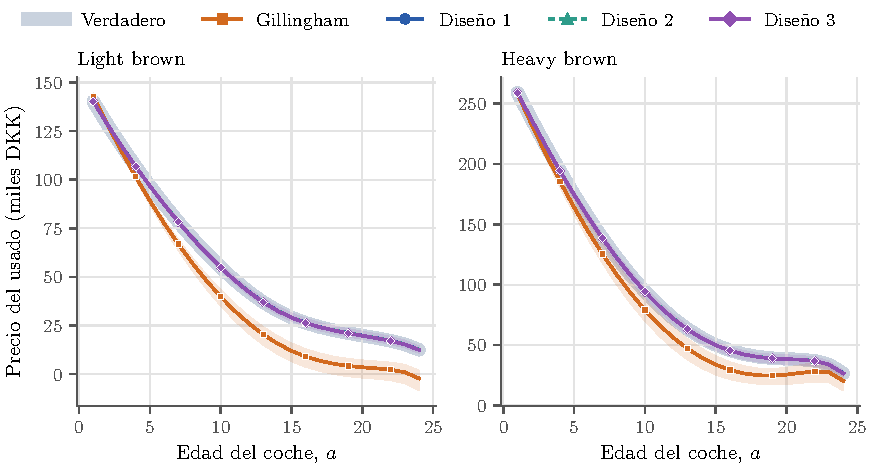
\includegraphics[width=\textwidth]{figuras/fig4_precios}
  \caption{...}\label{fig:precios}
\end{figure}
\end{verbatim}

%======================================================================
\section{Fuentes de datos y muestra}\label{sec:datos}

\subsection{Archivos que se leen}
Todo sale de la corrida \texttt{base} del Monte Carlo y del equilibrio verdadero \texttt{R\_LB}:

\begin{center}\small
\begin{tabular}{p{0.43\textwidth}p{0.5\textwidth}}
\toprule
Archivo (en \archivo{claude/niu/final/output/modelo_tesis/}) & Qué contiene \\
\midrule
\archivo{montecarlo/base/parametros_reps*.csv} &
  Una fila por (réplica, diseño, arranque, parámetro): \texttt{verdad}, \texttt{estimado} (en unidades
  naturales), \texttt{se} (error estándar BHHH), \texttt{ll}, \texttt{convergio}, \texttt{mejor}
  (si ese arranque es el de mayor verosimilitud). Lo escribe \archivo{montecarlo.py}. Hay un archivo
  por rango de réplicas (\archivo{0-499}, \archivo{158-499}, \archivo{500-999}, \ldots) porque
  la corrida se cortó y se reanudó. \\[3pt]
\archivo{montecarlo/base/gill_parametros_reps*.csv} &
  Lo mismo para el estimador de Gillingham (\texttt{gill\_completa}): 20 parámetros, sin $w$ ni $r$. \\[3pt]
\archivo{montecarlo/base/por_edad_mc.csv} &
  Para cada (réplica, diseño) se toma $\hat\theta$, se resuelve el equilibrio de los tres regímenes
  y se guardan agregados por (régimen, marca $j$, edad $a$): \texttt{q}, \texttt{P\_stock},
  \texttt{P\_transaccion}, \texttt{keep}, \texttt{reparar}, \texttt{w\_medio}. La fila con
  \texttt{rep}$=-1$, \texttt{estimador}=\texttt{verdad} es el equilibrio verdadero. Lo escribe
  \archivo{modelo_tesis/por_edad_mc.py}. \\[3pt]
\archivo{montecarlo/base/gill_por_edad_mc.csv} &
  Igual, para Gillingham: su equilibrio (un solo mercado, sin reparación) en su $\hat\theta$,
  por $(j,a)$: \texttt{q}, \texttt{P}, \texttt{keep}. Lo escribe \archivo{gillingham/por_edad_mc.py}. \\[3pt]
\archivo{teoria/R_LB/equilibrios.npz} &
  El vector $z=(EV_1,EV_2,P)$ del equilibrio verdadero de cada régimen (3 filas de 10{,}230). Lo
  escribe \archivo{teoria.py}; es el mismo que usa el Monte Carlo como verdad
  (\texttt{true\_equilibria} revisa que $\theta$ y el tamaño coincidan). \\
\bottomrule
\end{tabular}
\end{center}

\subsection{Qué filas se usan}\label{sec:filtros}
\begin{enumerate}
\item \textbf{Mejor arranque.} Solo las filas con \texttt{mejor = True}. En casi todas las réplicas hay
  un solo arranque (la verdad); en la réplica 0 hay además dos perturbados y se queda el de mayor $LL$.
\item \textbf{Una fila por (réplica, estimador, parámetro).} Los archivos se leen en orden alfabético
  (primero el rango original y después los de reanudación; los \archivo{*_faltantes} al final) y si una
  combinación aparece más de una vez se queda la \emph{última}. Esto pasa con Gillingham: cuando se
  detuvo la corrida, algunas réplicas ya tenían a Gillingham estimado y, al reanudar, se volvió a
  estimar. Las dos estimaciones son del mismo panel (semilla = réplica), así que da igual cuál se tome.
\item \textbf{Solo réplicas que convergieron} (\texttt{convergio = True}). Convergió el
  \ConvDuno\% de las réplicas en el diseño 1, el \ConvDdos\% en el 2, el \ConvDtres\% en el 3 y el
  \ConvGill\% en Gillingham.
\end{enumerate}
Con esto, las tablas 1 y 2 y la figura 3 usan las réplicas que se reportan en la nota de cada tabla.
En total hay \NrepsDuno{} réplicas estimadas por diseño y \NrepsGill{} de Gillingham.

\nota{Por ahora \archivo{por_edad_mc.csv} solo tiene las réplicas 0--59 (\NrepsEdad{} por diseño y
\NrepsEdadGill{} de Gillingham), porque los equilibrios por réplica se calculan al cerrar el Monte Carlo.
Las figuras 4, 5 y 6 usan esas réplicas. Cuando la estación de trabajo corra
\archivo{por_edad_mc.py} sobre todas las réplicas, basta volver a correr el script.}

\subsection{Notación}
Las marcas son \emph{light brown} (LB, $j=0$ en el código) y \emph{heavy brown} (HB, $j=1$); los tipos
son la pareja pobre ($\tau=1$, \texttt{t0}) y el soltero pobre ($\tau=2$, \texttt{t1}), cada uno con masa
$f_\tau=1/2$. Los regímenes son $R_m=R\,e^{\zeta_m}$ con $\zeta\in\{-0.3,0,0.3\}$ (reparación barata,
base y cara; \texttt{regimen} = 0, 1, 2). Un estimador $e$ en la réplica $k$ da $\hat\theta_{e,k}$;
$\theta_0$ es el valor verdadero y $K_e$ el número de réplicas que se usan.

%======================================================================
\section{Tablas 1 y 2: parámetros y sus sesgos}\label{sec:tablas}

\begin{table}[htbp]
\centering
\small
\setlength{\tabcolsep}{4.5pt}
\begin{adjustbox}{max width=\textwidth}
\begin{tabular}{l r rr rr rr rr}
\toprule
 & & \multicolumn{2}{c}{Gillingham} & \multicolumn{2}{c}{Diseño 1} & \multicolumn{2}{c}{Diseño 2} & \multicolumn{2}{c}{Diseño 3}\\
\cmidrule(lr){3-4} \cmidrule(lr){5-6} \cmidrule(lr){7-8} \cmidrule(lr){9-10}
Parámetro & Verdad & Media & Sesgo \% & Media & Sesgo \% & Media & Sesgo \% & Media & Sesgo \%\\
\midrule
\multicolumn{10}{l}{\textit{Preferencias}}\\
$\mu_{1}$ & 0.113 & 0.068 & \textbf{$-$39.9} & 0.113 & 0.2 & 0.113 & 0.3 & 0.114 & 0.4\\
$\mu_{2}$ & 0.094 & 0.058 & \textbf{$-$38.9} & 0.094 & 0.3 & 0.094 & 0.3 & 0.094 & 0.4\\
$u_{0,1\text{LB}}$ & 3.649 & 2.819 & \textbf{$-$22.7} & 3.654 & 0.1 & 3.655 & 0.2 & 3.657 & 0.2\\
$u_{0,1\text{HB}}$ & 5.154 & 3.626 & \textbf{$-$29.6} & 5.164 & 0.2 & 5.166 & 0.2 & 5.168 & 0.3\\
$u_{0,2\text{LB}}$ & 2.404 & 1.737 & \textbf{$-$27.7} & 2.410 & 0.2 & 2.411 & 0.3 & 2.413 & 0.4\\
$u_{0,2\text{HB}}$ & 3.582 & 2.338 & \textbf{$-$34.7} & 3.593 & 0.3 & 3.595 & 0.4 & 3.597 & 0.4\\
$u_{1,1\text{LB}}$ & $-$0.146 & $-$0.103 & \textbf{29.2} & $-$0.146 & $-$0.1 & $-$0.146 & $-$0.2 & $-$0.146 & $-$0.3\\
$u_{1,1\text{HB}}$ & $-$0.220 & $-$0.166 & \textbf{24.3} & $-$0.220 & $-$0.2 & $-$0.220 & $-$0.2 & $-$0.220 & $-$0.2\\
$u_{1,2\text{LB}}$ & $-$0.098 & $-$0.060 & \textbf{39.3} & $-$0.099 & $-$0.2 & $-$0.099 & $-$0.3 & $-$0.099 & $-$0.4\\
$u_{1,2\text{HB}}$ & $-$0.160 & $-$0.115 & \textbf{27.9} & $-$0.160 & $-$0.3 & $-$0.161 & $-$0.3 & $-$0.161 & $-$0.4\\
\addlinespace
\multicolumn{10}{l}{\textit{Costos de transacción}}\\
$T_{b,1}$ & 6.594 & 7.356 & \textbf{11.5} & 6.588 & $-$0.1 & 6.586 & $-$0.1 & 6.588 & $-$0.1\\
$T_{b,2}$ & 6.546 & 7.291 & \textbf{11.4} & 6.540 & $-$0.1 & 6.539 & $-$0.1 & 6.540 & $-$0.1\\
$T^{\emptyset}_{b,1}$ & 1.790 & 2.554 & \textbf{42.7} & 1.784 & $-$0.4 & 1.782 & $-$0.4 & 1.784 & $-$0.3\\
$T^{\emptyset}_{b,2}$ & 3.082 & 3.830 & \textbf{24.3} & 3.076 & $-$0.2 & 3.074 & $-$0.2 & 3.076 & $-$0.2\\
$T_s$ & 0.911 & $-$0.181 & \textbf{$-$119.9} & 0.916 & 0.6 & 0.918 & 0.8 & 0.916 & 0.6\\
$\sigma_D$ & 0.345 & 0.342 & $-$1.1 & 0.346 & 0.1 & 0.346 & 0.2 & 0.346 & 0.1\\
\addlinespace
\multicolumn{10}{l}{\textit{Accidentes}}\\
$\alpha_{0,\text{LB}}$ & $-$5.625 & $-$5.107 & \textbf{9.2} & $-$5.625 & 0.0 & $-$5.625 & 0.0 & $-$5.621 & 0.1\\
$\alpha_{0,\text{HB}}$ & $-$5.673 & $-$5.091 & \textbf{10.3} & $-$5.674 & 0.0 & $-$5.674 & 0.0 & $-$5.676 & $-$0.1\\
$\alpha_{1,\text{LB}}$ & 0.180 & 0.133 & \textbf{$-$26.1} & 0.180 & 0.0 & 0.180 & 0.0 & 0.180 & $-$0.3\\
$\alpha_{1,\text{HB}}$ & 0.202 & 0.208 & 3.2 & 0.202 & 0.1 & 0.202 & 0.1 & 0.202 & 0.1\\
\bottomrule
\end{tabular}
\end{adjustbox}
\caption{Parámetros que el modelo comparte con Gillingham et al.\ (2022): estimados del Monte Carlo}
\label{tab:mc-comunes}
\par\smallskip
\begin{minipage}{\textwidth}\footnotesize
\textit{Nota:} Gillingham se estima con su verosimilitud ``completa'' (observa el motivo de salida) sobre el mismo panel, sin $w$ ni $r$. Media de $\hat\theta$ entre réplicas;
sesgo \% $=100\,(\overline{\hat\theta}-\theta_0)/|\theta_0|$; en negritas, $|\text{sesgo}|\ge5\%$.
La desviación estándar entre réplicas está en la figura 3 y en \texttt{resumen\_parametros.csv}.
Réplicas: Gillingham: 448, Diseño 1: 456, Diseño 2: 456, Diseño 3: 457.
\end{minipage}
\end{table}

\begin{table}[htbp]
\centering
\small
\setlength{\tabcolsep}{4.5pt}
\begin{adjustbox}{max width=\textwidth}
\begin{tabular}{l r rr rr rr}
\toprule
 & & \multicolumn{2}{c}{Diseño 1} & \multicolumn{2}{c}{Diseño 2} & \multicolumn{2}{c}{Diseño 3}\\
\cmidrule(lr){3-4} \cmidrule(lr){5-6} \cmidrule(lr){7-8}
Parámetro & Verdad & Media & Sesgo \% & Media & Sesgo \% & Media & Sesgo \%\\
\midrule
\multicolumn{8}{l}{\textit{Preferencias}}\\
$u_w$ & $-$0.200 & $-$0.201$^{***}$ & $-$0.3 & $-$0.201$^{***}$ & $-$0.5 & $-$0.201$^{***}$ & $-$0.6\\
 &  & (0.007) &  & (0.009) &  & (0.010) & \\[1pt]
\addlinespace
\multicolumn{8}{l}{\textit{Desgaste}}\\
$\delta_{\text{LB}}$ & 0.075 & 0.075$^{***}$ & 0.0 & 0.075$^{***}$ & $-$0.1 & 0.075$^{***}$ & $-$0.2\\
 &  & (0.001) &  & (0.001) &  & (0.001) & \\[1pt]
$\delta_{\text{HB}}$ & 0.075 & 0.075$^{***}$ & 0.0 & 0.075$^{***}$ & $-$0.1 & 0.075$^{***}$ & $-$0.1\\
 &  & (0.001) &  & (0.001) &  & (0.001) & \\[1pt]
$\kappa$ & 0.250 & 0.250$^{***}$ & 0.0 & 0.250$^{***}$ & $-$0.1 & 0.250$^{***}$ & $-$0.1\\
 &  & (0.001) &  & (0.002) &  & (0.002) & \\[1pt]
$\sigma_\eta$ & 0.150 & 0.150$^{***}$ & 0.0 & 0.150$^{***}$ & 0.0 & 0.150$^{***}$ & 0.0\\
 &  & (0.000) &  & (0.001) &  & (0.001) & \\[1pt]
\addlinespace
\multicolumn{8}{l}{\textit{Reparación}}\\
$\sigma_r$ & 0.300 & 0.301$^{***}$ & 0.3 & 0.301$^{***}$ & 0.2 & 0.301$^{***}$ & 0.3\\
 &  & (0.009) &  & (0.011) &  & (0.012) & \\[1pt]
\bottomrule
\end{tabular}
\end{adjustbox}
\caption{Parámetros propios del modelo con reparación: estimados del Monte Carlo}
\label{tab:mc-propios}
\par\smallskip
\begin{minipage}{\textwidth}\footnotesize
\textit{Nota:} Gillingham no tiene estos parámetros. Media de $\hat\theta$ entre réplicas;
entre paréntesis, su desviación estándar entre réplicas (en unidades del parámetro).
Significancia de $\overline{\hat\theta}/\text{DE}$ contra cero (normal, dos colas):
$^{*}p<0.10$, $^{**}p<0.05$, $^{***}p<0.01$.
Sesgo \% $=100\,(\overline{\hat\theta}-\theta_0)/|\theta_0|$; en negritas, $|\text{sesgo}|\ge5\%$.
Réplicas: Diseño 1: 456, Diseño 2: 456, Diseño 3: 457.
\end{minipage}
\end{table}


\subsection{Qué parámetros van en cada tabla}
\textbf{Tabla~\ref{tab:mc-comunes}} tiene los 20 parámetros que existen en los dos modelos y que estima
Gillingham: $\mu_\tau$, $u_{0,\tau j}$, $u_{1,\tau j}$, $T_{b,\tau}$, $T^\emptyset_{b,\tau}$, $T_s$,
$\sigma_D$, $\alpha_{0j}$ y $\alpha_{1j}$. \textbf{Tabla~\ref{tab:mc-propios}} tiene los 6 que solo
existen en el modelo con reparación: $u_w$, $\delta_{\text{LB}}$, $\delta_{\text{HB}}$, $\kappa$,
$\sigma_\eta$ y $\sigma_r$; ahí no hay columna de Gillingham.

\subsection{Cálculos}
Para cada estimador $e$ y parámetro $p$, sobre las $K_e$ réplicas de la sección~\ref{sec:filtros}:
\begin{align*}
\text{Media} &= \overline{\hat\theta}_{e,p}=\frac1{K_e}\sum_{k}\hat\theta_{e,p,k},\qquad
\text{DE} = \sqrt{\frac1{K_e-1}\sum_k\big(\hat\theta_{e,p,k}-\overline{\hat\theta}_{e,p}\big)^2},\\
\text{Sesgo \%} &= 100\,\frac{\overline{\hat\theta}_{e,p}-\theta_{0,p}}{|\theta_{0,p}|}.
\end{align*}
Se divide entre $|\theta_0|$ (y no entre $\theta_0$) para que el signo del sesgo diga siempre si el
estimador sobreestima ($+$) o subestima ($-$), aunque el parámetro sea negativo (por ejemplo $u_{1,\tau j}$
o $\alpha_{0j}$). Los valores con $|\text{sesgo}|\ge5\%$ van en negritas: en la práctica son solo los
de Gillingham.

Los parámetros están en unidades naturales (las de la tabla de calibración de la tesis), aunque
$\mu_\tau$, $\kappa$, $\sigma_\eta$ y $\sigma_r$ se estimen en logaritmos: \archivo{montecarlo.py}
guarda $\hat\theta$ ya transformado y su error estándar con el método delta.

En \archivo{tablas/resumen_parametros.csv} están además
\begin{gather*}
\text{RMSE}=\sqrt{\tfrac1{K_e}\textstyle\sum_k(\hat\theta_{e,p,k}-\theta_{0,p})^2},\\
\text{cobertura}=\tfrac1{K_e}\textstyle\sum_k\mathbf 1\big\{|\hat\theta_{k}-\theta_{0}|\le1.96\,\widehat{se}_{k}\big\},
\end{gather*}
el error estándar mediano y la DE en \% de $|\theta_0|$. En los diseños 1--3 la cobertura de los
intervalos al 95\% va de \CobMin\% a \CobMax\% según el parámetro, es decir, los errores estándar BHHH
están bien calibrados.

\subsection{Lectura}
En los tres diseños el peor sesgo, sobre los 26 parámetros, es de \PeorSesgoD\% en valor absoluto.
Gillingham, en cambio, subestima la utilidad marginal del dinero ($\mu_1$: \Gillmutcero\%, $\mu_2$:
\Gillmutuno\%), y con ella las utilidades base ($u_{0,1\text{LB}}$: \Gillucerotcerojcero\%), y le
cambia el signo al costo del vendedor ($T_s$: \Gilltcsell\%). La pendiente de accidentes por edad
$\alpha_{1,\text{LB}}$ sale \Gillaccagejcero\%: su modelo atribuye al envejecimiento parte del deterioro
que en los datos depende de $w$ y de la reparación.

%======================================================================
\section{Figura 3: estimados centrados en el valor verdadero}

\setcounter{figure}{2}
\begin{figure}[H]
\centering
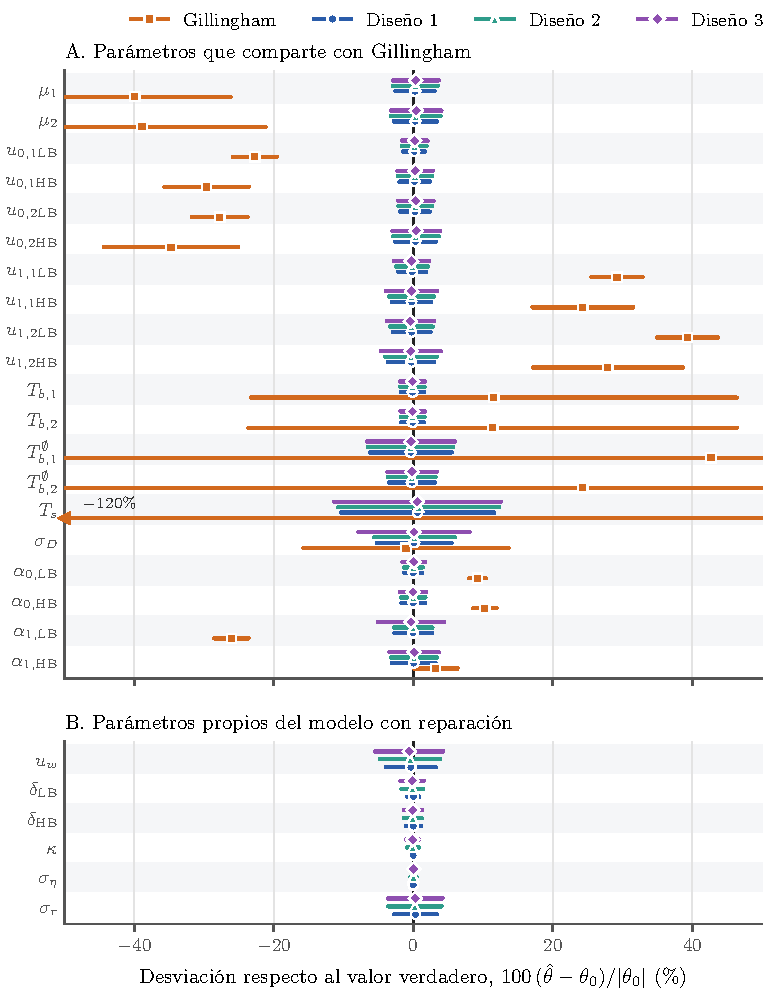
\includegraphics[width=\textwidth]{figuras/fig3_dispersion}
\caption{Distribución de los estimados alrededor del valor verdadero. El punto es la media entre
réplicas y la barra $\pm$ una desviación estándar, ambas en \% de $|\theta_0|$; la línea vertical en 0
es el valor verdadero. Las flechas marcan valores fuera de la escala.}
\label{fig:dispersion}
\end{figure}

\paragraph{Datos.} Las mismas réplicas y estadísticas que las tablas 1 y 2
(\archivo{parametros_reps*.csv} y \archivo{gill_parametros_reps*.csv}).

\paragraph{Cálculo.} Para que los 26 parámetros quepan en un mismo eje, todo se expresa como
desviación porcentual respecto al verdadero: el punto es el sesgo \%
$100(\overline{\hat\theta}-\theta_0)/|\theta_0|$ y la barra va de
$100(\overline{\hat\theta}-\theta_0-\text{DE})/|\theta_0|$ a $100(\overline{\hat\theta}-\theta_0+\text{DE})/|\theta_0|$.
Así, ``centrado en el valor verdadero'' es la línea en 0. Panel A: los 20 parámetros comunes (cuatro
estimadores); panel B: los 6 propios (tres diseños). El eje se corta en $\pm50\%$ para que se vean los
diseños; lo que se sale (el punto de $T_s$ de Gillingham, en \Gilltcsell\%, y parte de algunas barras
de Gillingham) se marca con una flecha en el borde y su valor.

\paragraph{Lectura.} Los diseños 1--3 están centrados en 0 en todos los parámetros; lo que cambia entre
diseños es el ancho de la barra: perder $r$ (diseño 2) y luego el motivo de salida (diseño 3) hace los
estimados más dispersos, pero no sesgados. Las barras más anchas son las de $T_s$, $\sigma_D$ y
$T^\emptyset_{b,\tau}$, que dependen de eventos relativamente raros en el panel (ventas, chatarreo
voluntario y compras desde sin coche).
Gillingham está desplazado del cero en casi todo: es el sesgo de ignorar la reparación (sus valores
pseudo-verdaderos), no ruido.

%======================================================================
\section{Figura 4: precios estimados y verdaderos}

\begin{figure}[H]
\centering
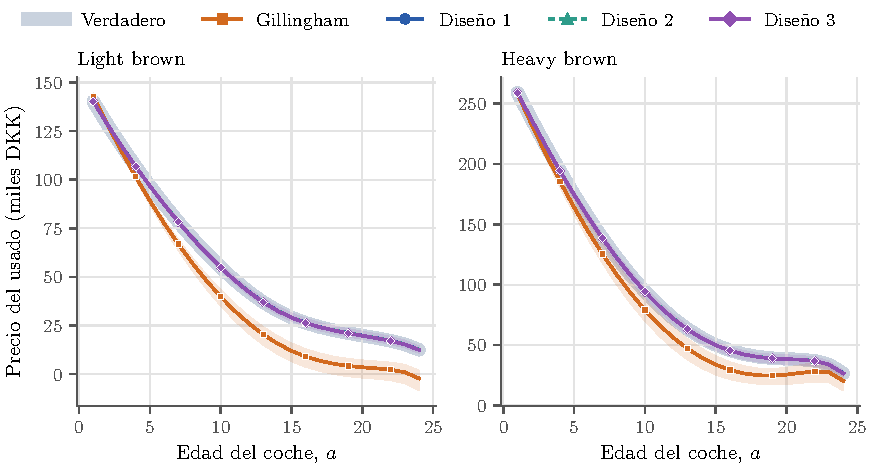
\includegraphics[width=\textwidth]{figuras/fig4_precios}
\caption{Precio promedio del coche usado por edad en el régimen base. Banda gris: equilibrio verdadero.
Líneas: media entre réplicas del precio de equilibrio en $\hat\theta$; sombreado: percentiles
2.5--97.5 entre réplicas (diseño 3 y Gillingham).}
\label{fig:precios}
\end{figure}

\paragraph{Datos.} \archivo{por_edad_mc.csv} (verdad y diseños 1--3, columna \texttt{P\_transaccion},
\texttt{regimen}$=1$) y \archivo{gill_por_edad_mc.csv} (Gillingham, columna \texttt{P}, filas
\texttt{estimador = gill\_completa}).

\paragraph{Cómo se generó \texttt{por\_edad\_mc.csv}.} Para cada réplica $k$ y diseño $e$,
\archivo{por_edad_mc.py} arma $\hat\theta_{e,k}$ y resuelve el equilibrio $(EV_1,EV_2,P)$ de cada
régimen con el método de cuerda, arrancando en el equilibrio verdadero corregido con la derivada
$dz/d\theta$ ($z_0+\tfrac{dz}{d\theta}(\hat\theta-\theta_0)$). Si algún régimen no converge, la
réplica se omite (no pasó en ninguna). Con el equilibrio calcula, para cada tipo, las probabilidades
de elección y la distribución estacionaria $q_\tau(x)$, y agrega por $(j,a)$ con
\texttt{equilibrium.by\_age}. El precio de equilibrio $P(j,a,w)$ depende del desgaste, así que para tener
un precio por $(j,a)$ se promedia sobre $w$ con el peso de los coches que \emph{se ofrecen} en el mercado:
\begin{gather*}
\bar P(j,a)=\frac{\sum_w S(j,a,w)\,P(j,a,w)}{\sum_w S(j,a,w)},\\
S(x)=\sum_\tau f_\tau\,q_\tau(x)\,\big[1-k_\tau(x)\big]\big[1-c_\tau(x)\big],\qquad x=(j,a,w),
\end{gather*}
donde $k_\tau(x)$ es la probabilidad de quedarse el coche y $c_\tau(x)$ la de chatarrizarlo si se deshace de él,
así que $\bar P$ es el precio promedio de las transacciones (\texttt{P\_transaccion}). Se usa este y no el
promedio sobre el stock porque es el comparable con el precio de Gillingham, que es el precio al que se
intercambia un coche $(j,a)$ (en su modelo no hay $w$). Es el mismo que usa el póster.

Gillingham: \archivo{gillingham/por_edad_mc.py} resuelve el equilibrio de \emph{su} modelo
(sin $w$, sin reparación, un solo mercado) en su $\hat\theta$ y guarda $P(j,a)$.

\paragraph{Cálculo de la figura.} Por estimador y $(j,a)$: media de $\bar P(j,a)$ entre réplicas
(línea) y percentiles 2.5 y 97.5 (sombra). La banda gris gruesa es la verdad; la línea negra delgada
dentro de ella marca el valor exacto. Un panel por marca.

\paragraph{Lectura.} Los tres diseños quedan encima de la verdad (el mayor error en la media es de
\ErrPrecioD\%, en cualquier edad y marca). Gillingham da precios cerca del verdadero en el coche de un
año (\ErrPrecioGillJoven\% en LB) pero cada vez más bajos con la edad: su modelo no sabe que los
coches viejos que siguen en el mercado son los que se han reparado, y llega a precios negativos en la
última edad de LB.

%======================================================================
\section{Figura 5: distribución de la población}

\begin{figure}[H]
\centering
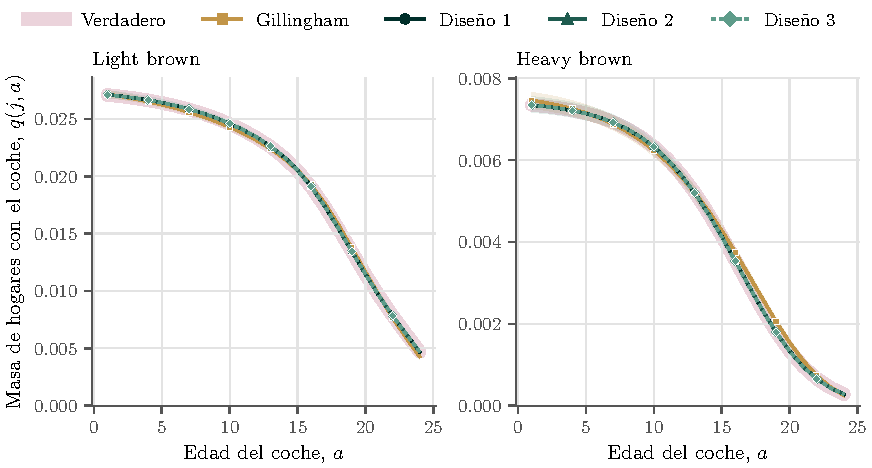
\includegraphics[width=\textwidth]{figuras/fig5_poblacion}
\caption{Distribución estacionaria de coches por marca y edad en el régimen base: masa de hogares que
empieza el año con un coche $(j,a)$. Mismas convenciones que la figura~\ref{fig:precios}.}
\label{fig:poblacion}
\end{figure}

\paragraph{Datos.} Columna \texttt{q} de \archivo{por_edad_mc.csv} (\texttt{regimen}$=1$) y de
\archivo{gill_por_edad_mc.csv}.

\paragraph{Cálculo.} $q(j,a)=\sum_\tau f_\tau\sum_w q_\tau(j,a,w)$: la masa (de entre 1, la población
de hogares) que empieza el año con un coche de marca $j$ y edad $a$, sumando los dos tipos con sus pesos
$f_\tau=1/2$ y todos los niveles de desgaste. Lo que falta para sumar 1 son los hogares sin coche y los
que tienen un coche en estado terminal. En Gillingham es lo mismo pero sin $w$. Media entre réplicas
y percentiles 2.5--97.5 igual que en la figura 4.

\paragraph{Lectura.} La distribución por edad casi no se mueve: aun Gillingham la reproduce bien. Esto es
de esperar, porque su estimador ajusta las frecuencias de mantener, vender y comprar por $(j,a)$, que
son justo lo que determina $q(j,a)$. Su sesgo aparece en los precios (figura 4) y en los parámetros
(tablas), no en las cantidades.

%======================================================================
\section{Figura 6: probabilidad de reparar por edad y diseño}

\begin{figure}[H]
\centering
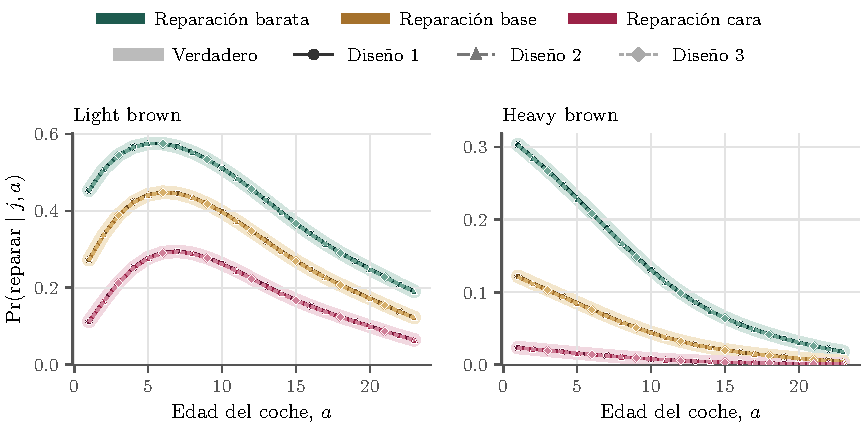
\includegraphics[width=\textwidth]{figuras/fig6_reparar_edad}
\caption{Probabilidad de reparar por edad, verdadera y en el equilibrio de cada diseño estimado. Filas:
regímenes de precio de reparación; columnas: marcas. Sombreado: percentiles 2.5--97.5 del diseño 3.
Nótese que la escala vertical cambia entre paneles.}
\label{fig:reparar-edad}
\end{figure}

\paragraph{Datos.} Columna \texttt{reparar} de \archivo{por_edad_mc.csv}, los tres regímenes.
Gillingham no tiene reparación, así que no aparece.

\paragraph{Cálculo.} En el modelo la decisión de reparar se toma para cada tenencia $(j,a,w)$ con
probabilidad $\Pi_\tau(r{=}1\mid j,a,w)=\Lambda\big((v_1-v_0)/\sigma_r\big)$ (la etapa 2 de
\texttt{bellman.repair\_stage}). Para tener una por $(j,a)$, \texttt{by\_age} la promedia sobre $w$ y tipos
con el peso de la distribución estacionaria:
\[
\Pr(\text{reparar}\mid j,a)=\frac{\sum_\tau f_\tau\sum_w q_\tau(j,a,w)\,\Pi_\tau(r{=}1\mid j,a,w)}
{\sum_\tau f_\tau\sum_w q_\tau(j,a,w)} .
\]
Esto se hace en la verdad y en el equilibrio de cada $\hat\theta$; la figura grafica la media entre
réplicas. Se omite la edad 24, en la que no se puede reparar (el coche llega a la edad terminal el año
siguiente y la probabilidad es 0 por construcción).

\nota{El peso es $q$, los coches al \emph{empezar} el año (antes de comerciar), porque así lo guarda
\texttt{by\_age}. Estrictamente la reparación la deciden las tenencias \emph{después} de comerciar
(los que se quedaron su coche más los que compraron uno usado). La diferencia es pequeña y es la misma en
la verdad y en los estimados, así que no afecta la comparación. La figura 8 sí usa tenencias.}

\paragraph{Lectura.} Los tres diseños recuperan la curva verdadera en todas las combinaciones. La forma
(una U invertida en LB y decreciente en HB) viene de los precios de reparación: en LB los coches
jóvenes tienen una prima en el precio de reparar. Al pasar de reparación barata a cara la probabilidad cae
en todas las edades: es la variación que da la variable excluida. La banda del diseño 3 es más ancha
en HB con reparación cara, donde casi nadie repara y hay pocas transiciones con las que separar la mezcla.

%======================================================================
\section{Figura 7: lo que se observa y lo que no}

\begin{figure}[H]
\renewcommand{\thefigure}{7a}
\centering
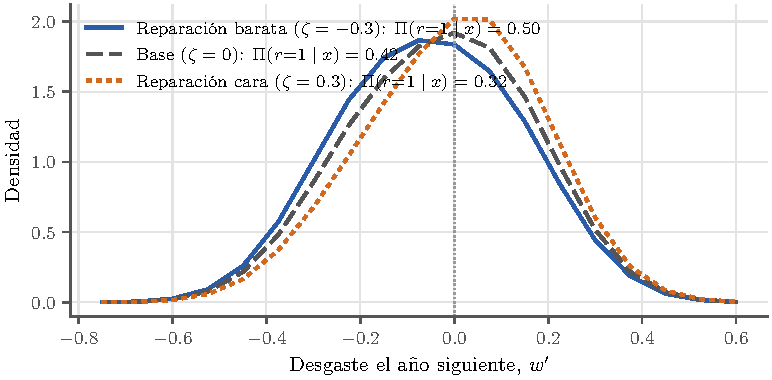
\includegraphics[width=\textwidth]{figuras/fig7a_mezcla_observada}
\caption{Distribución \emph{observada} del desgaste del año siguiente, $Z(w'\mid x)$, para un mismo
estado $x$ (light brown, edad 8, $w=0$) en los tres regímenes de precio de reparación.}
\label{fig:mezcla}
\end{figure}

\addtocounter{figure}{-1}
\begin{figure}[H]
\renewcommand{\thefigure}{7b}
\centering
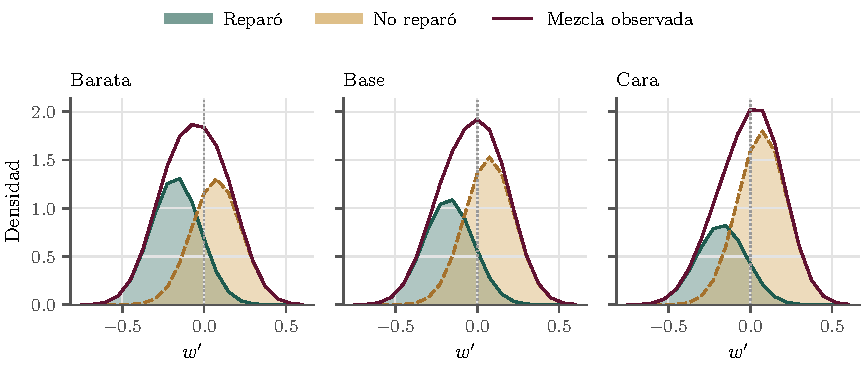
\includegraphics[width=\textwidth]{figuras/fig7b_componentes}
\caption{La misma distribución separada según la decisión de reparar, que el econometrista no ve. Azul:
coches que se repararon; naranja: los que no; línea negra: la suma, que es la curva de la
figura~\ref{fig:mezcla}.}
\label{fig:componentes}
\end{figure}

\paragraph{Datos.} El equilibrio verdadero de \archivo{teoria/R_LB/equilibrios.npz}. No usa el Monte
Carlo: son las densidades exactas del modelo (sin ruido de muestra), por eso las curvas son
lisas.\footnote{Lo ``observado'' quiere decir lo que vería el econometrista con muestra infinita.}

\paragraph{Cálculo.} El script carga $z_m$ de cada régimen, lo parte en $(EV_1,EV_2,P)$ y llama
\texttt{equilibrio.equilibrium\_objects}, que para cada tipo da las CCPs (incluida
$\Pi_\tau(r{=}1\mid h)$), la distribución estacionaria $q_\tau$ y la matriz de transición del desgaste
$F[r,j,w,w']$. Esta última es la masa de $N\big(w+\delta_j-\kappa r,\ \sigma_\eta^2\big)$ en cada celda del
grid de $w'$ (\texttt{bellman.w\_transition}); dividida entre el paso del grid ($\Delta=0.075$) es la densidad
$f(w'\mid x,r)$.

Se fija el estado $x=(j,a,w)=(\text{LB},8,0)$: una marca y edad con mucha masa y un $w$ (el de un coche
nuevo) que existe en los tres regímenes. Como el tipo de hogar sí se observa pero aquí queremos una sola
curva por régimen, la probabilidad de reparar junta los dos tipos con el peso de cuántos coches tiene
cada uno en ese estado:
\begin{gather*}
\Pi_m(r{=}1\mid x)=\frac{\sum_\tau f_\tau\,h_{\tau m}(x)\,\Pi_{\tau m}(r{=}1\mid x)}{\sum_\tau f_\tau\,h_{\tau m}(x)},\\
h_{\tau}(x)=q_\tau(x)\,k_\tau(x)+M_\tau\,b_\tau(x),
\end{gather*}
donde $h_\tau$ son las tenencias después de comerciar (quien se quedó su coche más quien compró ese usado),
$k_\tau(x)$ la probabilidad de quedarse el coche, $b_\tau(x)$ la de comprar el usado $x$ entre quienes
cambian de coche y $M_\tau=\sum_{x'} q_\tau(x')\Pr_\tau(\text{trade}\mid x')$ la masa que cambia. Con esto:
\begin{itemize}
\item Figura~\ref{fig:mezcla}: $Z_m(w'\mid x)=\Pi_m(1\mid x)\,f(w'\mid x,1)+\Pi_m(0\mid x)\,f(w'\mid x,0)$, una curva por régimen.
\item Figura~\ref{fig:componentes}: un panel por régimen con los dos sumandos por separado (áreas) y su suma (línea negra).
\end{itemize}
Las probabilidades que resultan son $\Pi(r{=}1\mid x)=\PiBarata$ (barata), \PiBase{} (base) y
\PiCara{} (cara). El efecto de reparar no depende del régimen: las densidades $f(w'\mid x,r)$ son las mismas en los tres
(medias $w+\delta_j=0.075$ sin reparar y $w+\delta_j-\kappa=-0.175$ reparando); solo cambian los pesos.

\nota{Condicionar en que el coche sobrevive no cambia nada aquí: en la especificación vigente la
probabilidad de avería $s(j,a,w)$ depende del $w$ de hoy y no de $r$, así que los coches que se
averían salen igual de los que reparan y de los que no.}

\paragraph{Lectura.} Es el argumento de identificación de Hu \& Xin en una imagen: el econometrista ve
la figura~\ref{fig:mezcla}, en la que al abaratar la reparación la masa se corre a la izquierda. Como el
precio de reparar mueve los pesos pero no las dos densidades de la figura~\ref{fig:componentes}, con dos
o más regímenes se pueden separar los componentes y recuperar $\kappa$, $\delta_j$, $\sigma_\eta$ y la
probabilidad de reparar.

%======================================================================
\section{Figura 8: probabilidad de reparar según el desgaste}

\begin{figure}[H]
\centering
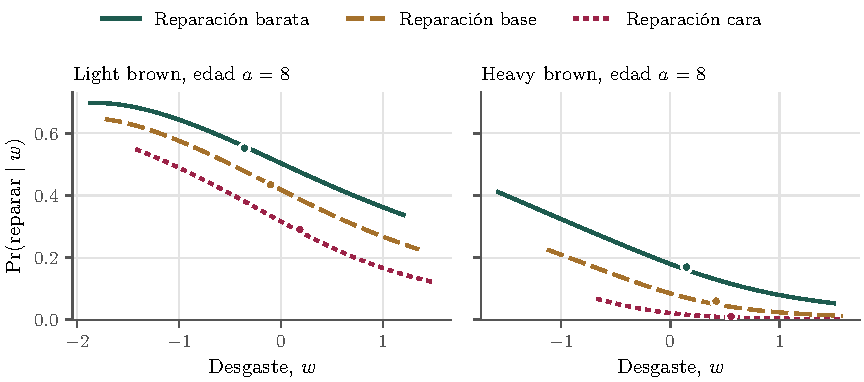
\includegraphics[width=\textwidth]{figuras/fig8_reparar_desgaste}
\caption{Probabilidad verdadera de reparar como función del desgaste, a edad 8, en cada régimen. El
punto marca el desgaste medio y la tasa promedio de los coches de esa marca y edad en cada régimen.}
\label{fig:reparar-w}
\end{figure}

\paragraph{Datos.} El mismo equilibrio verdadero que la figura 7 (\archivo{teoria/R_LB/equilibrios.npz}).

\paragraph{Cálculo.} Para cada régimen $m$, marca $j$ y $w$ del grid, con la edad fija en $a=8$:
\[
\Pr\nolimits_m(\text{reparar}\mid j,a,w)=\frac{\sum_\tau f_\tau\,h_{\tau m}(j,a,w)\,\Pi_{\tau m}(r{=}1\mid j,a,w)}{\sum_\tau f_\tau\,h_{\tau m}(j,a,w)},
\]
con las tenencias $h_{\tau m}$ de la figura 7 como pesos entre tipos. Se dibuja solo donde está el 99\%
central de los coches de esa $(j,a)$ en ese régimen (se cortan las colas de $w$ en las que casi no hay
coches), y por eso las tres curvas cubren rangos distintos: con reparación barata los coches están menos
desgastados. El punto es $\big(\bar w,\ \overline{\Pr}\big)$, el promedio de $w$ y de la probabilidad con
el peso de esas tenencias.

Se fija la edad porque, si se juntan todas, la curva mezcla el efecto de $w$ con la composición por edad
(a cada $w$ le corresponde una mezcla distinta de edades, y la probabilidad de reparar cambia mucho con la
edad, figura 6): sale una curva con quiebres que no son el efecto del desgaste.

\paragraph{Efecto de un cambio en el desgaste.} Para resumir la pendiente se calcula
$\frac{d\Pr}{dw}$ por diferencias finitas en el grid y se promedia con el peso de las tenencias; multiplicada
por 0.1 (dos tercios de $\sigma_\eta$) da el cambio en la probabilidad de reparar si el desgaste sube 0.1:

\begin{center}\small
\begin{tabular}{lccc}
\toprule
 & Barata & Base & Cara\\
\midrule
Light brown, $a=8$ & \PendLBBarata & \PendLBBase & \PendLBCara\\
Heavy brown, $a=8$ & \PendHBBarata & \PendHBBase & \PendHBCara\\
\bottomrule
\end{tabular}
\end{center}

\paragraph{Lectura.} Para un mismo coche, el precio de reparar desplaza toda la curva: es la variable
excluida. Dentro de un régimen, la probabilidad de reparar \emph{baja} con el desgaste. La razón está en
el modelo: reparar cuesta $\mu_\tau R$ hoy y baja $w'$ en $\kappa$ sin importar el $w$ de hoy, pero ese
beneficio solo se cobra si el coche sobrevive, y la probabilidad de sobrevivir, $1-s(j,a,w)$, baja con
el desgaste. Un coche muy desgastado probablemente se averíe antes de aprovechar la reparación. En HB con reparación cara casi nadie repara
en ningún nivel de desgaste.

%======================================================================
\section{Decisiones que tomé y dudas para ti}

\begin{enumerate}
\item \textbf{Gillingham ``completa''.} El único estimador de Gillingham en la corrida \texttt{base} es
  el que observa el motivo de salida (\texttt{gill\_completa}); la versión ``parcial'' del paper ya no se
  corre (no identifica las preferencias con estos datos). La tesis todavía menciona los dos en la tabla
  de estimadores.
\item \textbf{Columnas de las tablas.} Puse Media y Sesgo \% por estimador para que la tabla 1 (cuatro
  estimadores) quepa a lo ancho de la página con letra legible. La DE se ve en la figura 3; la DE, el RMSE,
  el error estándar mediano y la cobertura están en el CSV. Si quieres alguna en la tabla, se agrega en
  la función \texttt{tabla} del script (para la tabla 1 convendría ponerla en horizontal).
\item \textbf{Régimen de las figuras 4 y 5.} Uso el régimen base. Los otros dos se ven igual (los diseños
  sobre la verdad); si los quieres, es cambiar \texttt{regimenes=(1,)} por \texttt{(0,1,2)}.
\item \textbf{Estado de la figura 7.} Elegí $(\text{LB}, a=8, w=0)$. Se puede cambiar en la llamada
  \texttt{fig\_mezcla(cfg, reg, j=0, d=8, w=0.0)}.
\item \textbf{Edad de la figura 8.} $a=8$; con \texttt{fig\_rep\_w(cfg, reg, d\_fijo=...)} se cambia.
\item \textbf{Ojo con la tesis:} en la sección de calibración, \archivo{tesis.tex} dice
  $R_{\text{HB},a}=10+0.6(a-1)$, pero el código (y por tanto el Monte Carlo) usa un precio constante de
  16.6 para HB (\archivo{params.py}, \texttt{R\_BASE}: el promedio de esa recta en las edades 1--23).
  Hay que actualizar el texto.
\end{enumerate}

\end{document}
